\section{Tema 2: Verificación de equipos de medida eléctricos}
\subsection{Definiciones}
\begin{enumerate}
	\item \underline{\textbf{Patrón}}: Medida de referencia destinada a definir una unidad de una magnitud. Se usa para detectar desviaciones en aparatos al verificarlos respecto al patrón.
	\item \underline{\textbf{Patrón primario}}: Patrones iniciales con los que se comparan los patrones secundarios. Uso muy restringido, destinado a los  centros nacionales de metrología.
	\item \underline{\textbf{Patrón secundario}}: Se calibran con patrones primarios. Son menos precisos. Se emplean en laboratorios acreditados. 
	\item \underline{\textbf{Patrón industrial}}: Se calibran con patrones secundarios. Uso en control de calidad. 
	\item \underline{\textbf{Trazabilidad}}: Resultado de una medición que puede relacionarse con patrones de nivel más alto por medio de una cadena de comparaciones. Permite verificar un resultado.
	\item \underline{\textbf{Calibración}}: Operación que establece la relación entre los valores indicados por un patrón y el instrumento a calibrar. 
	\item \underline{\textbf{Verificación}}: Operación con el fin de comprobar que un instrumento cumple sus especificaciones.
	\item \underline{\textbf{Ajuste}}: Acción correctora para evitar que los resultados queden fuera de los valores admisibles.
\end{enumerate}
\subsection{Cualidades de los aparatos de medida patrones}
Están restringidos a laboratorios y centros nacionales de calibración. Tiene las siguientes características:
\begin{itemize}
 \item Exactitud muy elevada
 \item Alta sensibilidad, resolución y linealidad
 \item Deriva temporal pequeña
 \item Alta transparencia	
\end{itemize}
\newpage
En función de la magnitud a medir existen distintos patrones.
\begin{itemize}
		\item \underline{\textbf{Patrones de fuerza electromotriz}}: Se emplean para medir tensiones con baja incertidumbre.
		\begin{enumerate}
			\item \underline{Pila Weston}:
			\begin{itemize}
				\item Primer patrón de referencia.
					\item Su f.e.m es muy estable en el tiempo.
						\item  Tiene deriva térmica.
						\item  Si suministran corriente su f.e.m varia.
			\end{itemize} 
			\item \underline{Diodos Zener}:
			\begin{itemize}
				\item Tensiones más estables.
				\item Independiente de la temperatura.
			\end{itemize} 
			
			\begin{figure}[H]
				\centering
				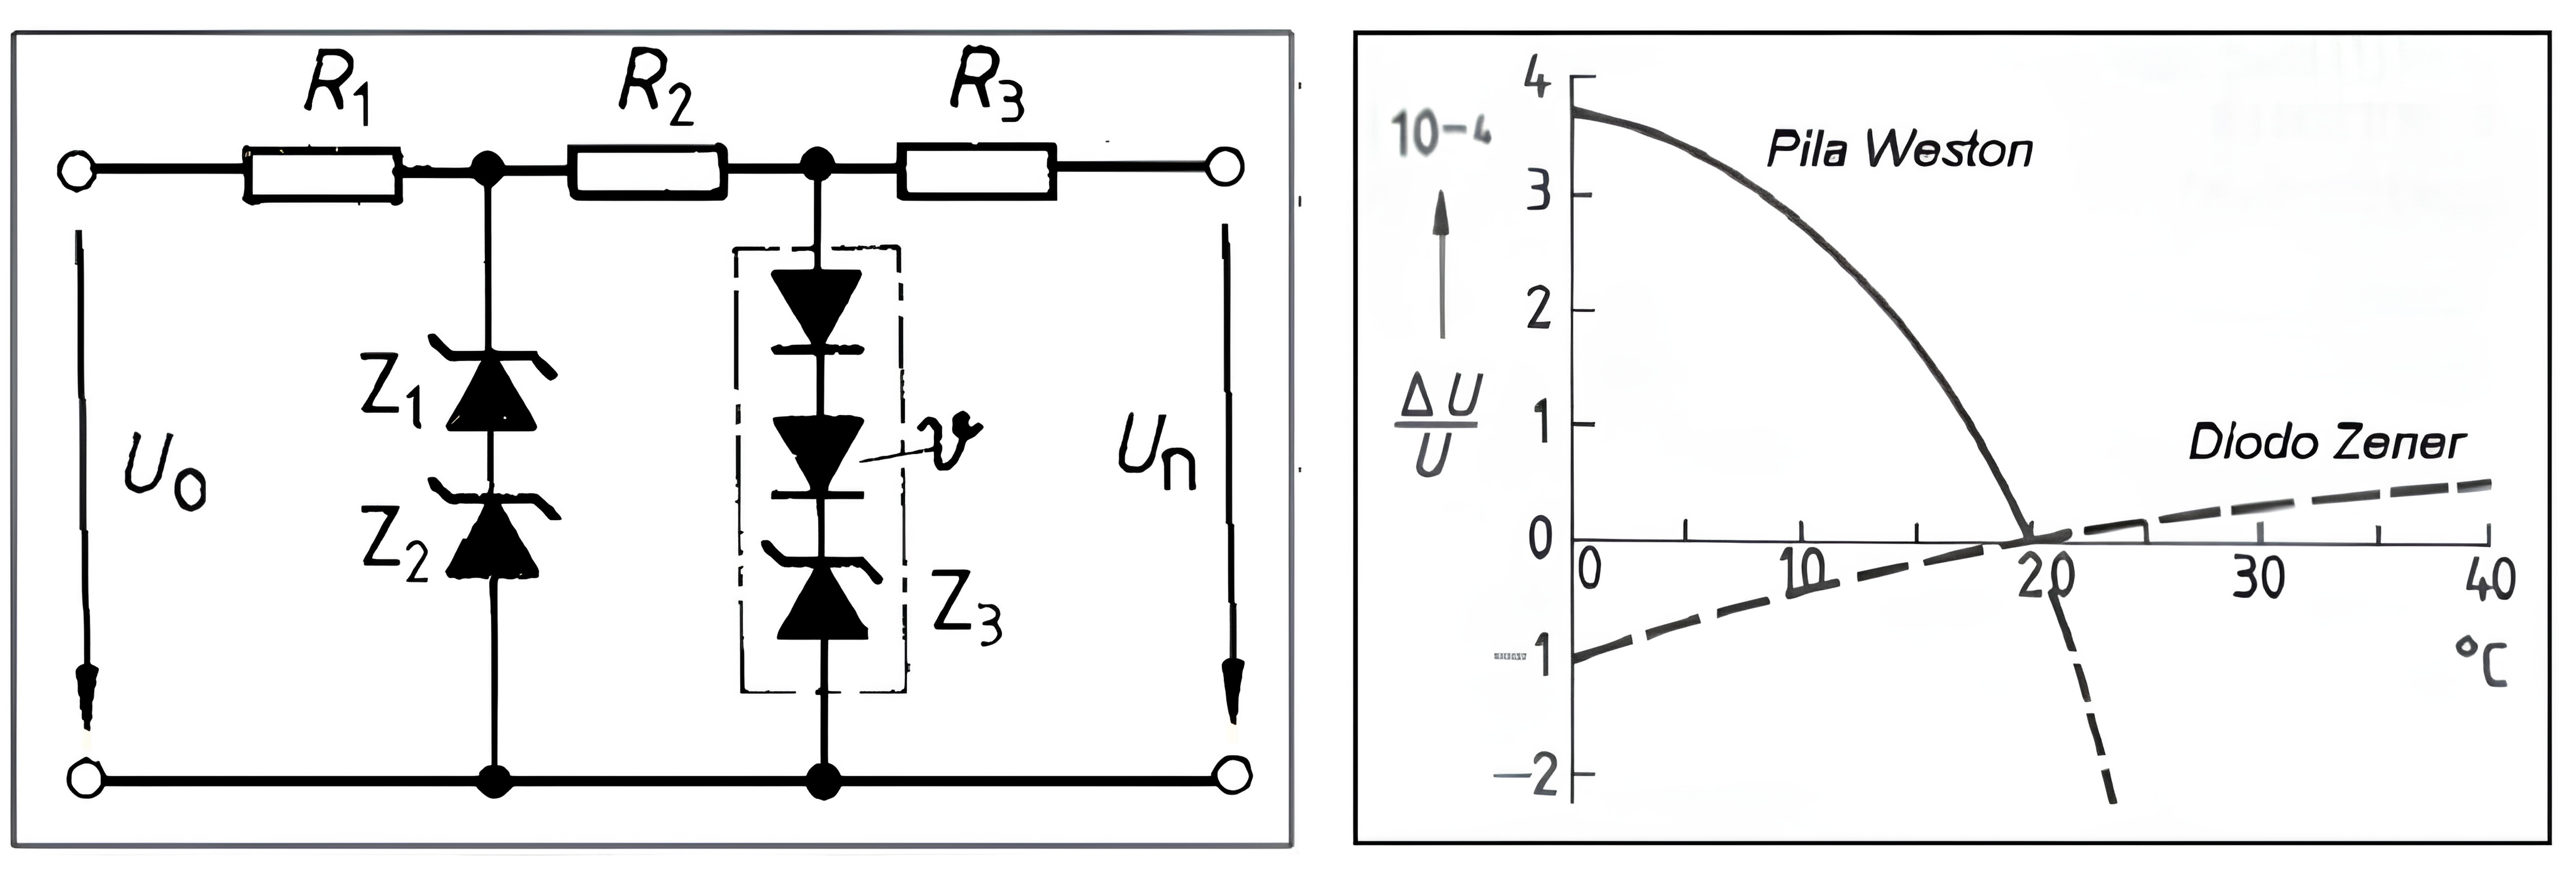
\includegraphics[width=0.5\textwidth]{imagenesTema2/zener.png}  
				\caption{Patrón Zener}
				\label{fig:sample}
			\end{figure}
	
		\end{enumerate}
	\item \underline{\textbf{Patrones de resistencia}}: Su clase corresponde a la diferencia en porcentaje entre el valor real y nominal.
	\begin{flushleft}
		Propiedades:
	\end{flushleft}
	\begin{itemize}
		\item Buena respuesta en frecuencia.
		\item Coeficiente de temperatura bajo.
		\item f.e.m térmica con el cobre baja.
		\item Elevada resistencia mecánica.
	\end{itemize}
	\begin{flushleft}
		Tipos:
	\end{flushleft}
	
	\begin{enumerate}
		\item \underline{Arrollamiento bifilar}: Tiene poca autoinducción, pero presenta elevada capacidad entre conductores. Se emplea para resistencias menores a 100 $\Omega$.
		
		\begin{figure}[H]
			\centering
			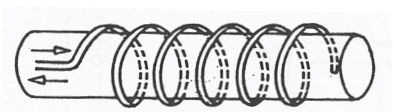
\includegraphics[width=0.5\linewidth]{imagenesTema2/bifilar}
			\caption{Arrollamiento bifilar}
			\label{fig:bifilar}
		\end{figure}
		
		\item \underline{Arrollamiento de Wagner}: Se divide en secciones para reducir la tensión entre espiras y la capacidad. Se bobina en sentido inverso para reducir la autoinducción. Se fabrican para más de 100 $\Omega$ y hasta unos 100 kHz.
		
		\begin{figure}[H]
			\centering
			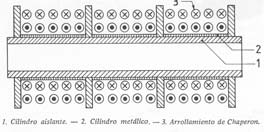
\includegraphics[width=0.5\linewidth]{imagenesTema2/ResisWagner}
			\caption{Arrollamiento Wagner}
			\label{fig:resiswagner}
		\end{figure}
		
		\item \underline{Caja de décadas}: Su capacidad de ajuste es muy elevada. Resistencias mayores a 10 $k\Omega$ en saltos de múltiplos de 10.
		\begin{figure}[H]
			\centering
			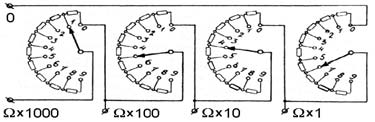
\includegraphics[width=0.5\linewidth]{imagenesTema2/decadas}
			\caption{Caja de décadas}
			\label{fig:decadas}
		\end{figure}
		
		
	\end{enumerate}
	
	\item \underline{\textbf{Patrones de inductancia}}: Autoinducción independiente del medio. Baja resistencia óhmnica  y bajo coeficiente de temperatura.
	
	\begin{figure}[H]
		\centering
		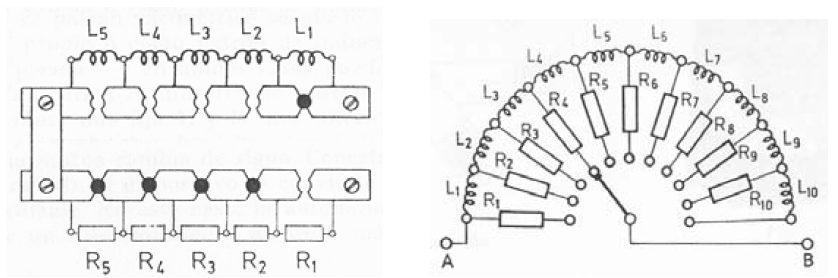
\includegraphics[width=0.5\linewidth]{imagenesTema2/inductancias}
		\caption{Patrones de inductancia}
		\label{fig:inductancias}
	\end{figure}
	
	\item \underline{\textbf{Patrones de capacidad}}: Deben reunir las siguientes características: 
	\begin{enumerate}
		\item Gran inmunidad a los campos electromagnéticos ajenos al medio.
		\item Mínima variación a lo largo del tiempo y por efecto de la temperatura.
		\item Capacidad independiente de la frecuencia.
		\item Ángulo de pérdidas bajo: por tener una resistencia interna.
		
	\end{enumerate}
	
	\begin{figure}
	\begin{subfigure}{0.5\textwidth}
		\centering
		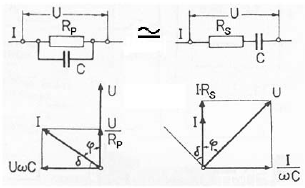
\includegraphics[width=\linewidth, height=1.5in, valign=t]{imagenesTema2/C1}
		\caption{Ángulo de pérdidas $tg(\delta)$}
		\label{fig:c1}
	\end{subfigure}
	\begin{subfigure}{0.5\textwidth}
		\centering
		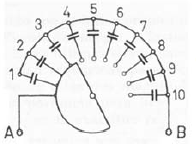
\includegraphics[width=\linewidth, height=1.5in, valign=t]{imagenesTema2/C2}
		\caption{Caja de décadas capacitiva}
		\label{fig:c2}
	\end{subfigure}
\end{figure}	
\end{itemize}
\subsection{Verificación de un aparato de medida}
Por la presencia de ruido o por el envejecimiento de los instrumentos de medida empiezan a aparecer defectos y es necesaria su calibración.
\begin{itemize}
	\item La principal causa de incertidumbre proviene del aparato a contrastar (Incertidumbre tipo B).
	\item  La mayor componente de tipo B la introduce el patrón.
	\item La magnitud debe ser ajustable en el rango del equipo a examen.
	\item Procedimiento:
	\begin{enumerate}
		\item Los aparatos se montan para que queden sometidos por igual a la magnitud.
		\item La magnitud se varia a intervalos regulares de modo que sus indicaciones sean siempre divisiones exactas.
		\item Los valores del patrón son los verdaderos.
		\item La diferencia entre las lecturas de los aparatos son las desviaciones.
		\item En cada punto se calcula la desviación típica y la media.
		\item Se elabora un gráfico de correcciones y se elabora un gráfico de calibración.
		\item Conviene repetir al menos diez veces las medidas, cinco en sentido ascendente y cinco en sentido descendente para evitar la histérisis.
		\item Obtener la incertidumbre de contratación.
	\end{enumerate}
\end{itemize}
\newpage
\subsection{Criterio de rechazo de Chauvenet}
Se emplea para discriminar datos erróneos fruto de despistes o un error en la toma de datos. Por ello, para evitar distorsiones se supone que los resultados siguen una distribución normal y se rechazan todas las medidas que verifiquen (proceso recursivo):

\[\lvert x_i - \bar x  \rvert> K(n) \hat{s}\]

\renewcommand{\arraystretch}{1.1} %
\begin{table}[H]
	\centering
	\begin{tabular}{|c|c|c|c|c|c|c|c|c|c|}
		\hline
		\textbf{n} &  2 & 3& 4& 5& 6& 7& 8& 9& 10 \\
		\hline
		\textbf{K(n)} &  1.15 & 1.38& 1.54& 1.65& 1.73& 1.80& 1.86& 1.92&1.96\\
		\hline
		\textbf{n} &11& 12& 13& 14& 15& 20& 30& 50& 100\\
		\hline
		
		\textbf{K(n)} & 2.00& 2.04& 2.07& 2.10& 2.13& 2.24& 2.40& 2.57& 2.81\\
		\hline
	\end{tabular}
	\caption{Tabla factor K(n)}
	\label{tab:example}
\end{table}

\subsection{Resultados de una verificación}
Se emplean gráficos de diferencias para mostrar la linealidad y el sesgo.

\[\text{Diferencia = Lectura del aparato a verificar - lectura del patrón}\]
\[\text{Corrección = - Diferencia}\]
\begin{enumerate}
	\item \underline{\textbf{Curva de diferencias absolutas}}: Da la corrección a introducir en las lecturas del aparato contrastado. \textbf{No debe unirse el cero de la escala con el primer punto de la calibración} para no asumir un error en una zona de alta incertidumbre.
	\[\text{Medida = lectura + corrección}\]
\begin{figure}[H]
	\centering
	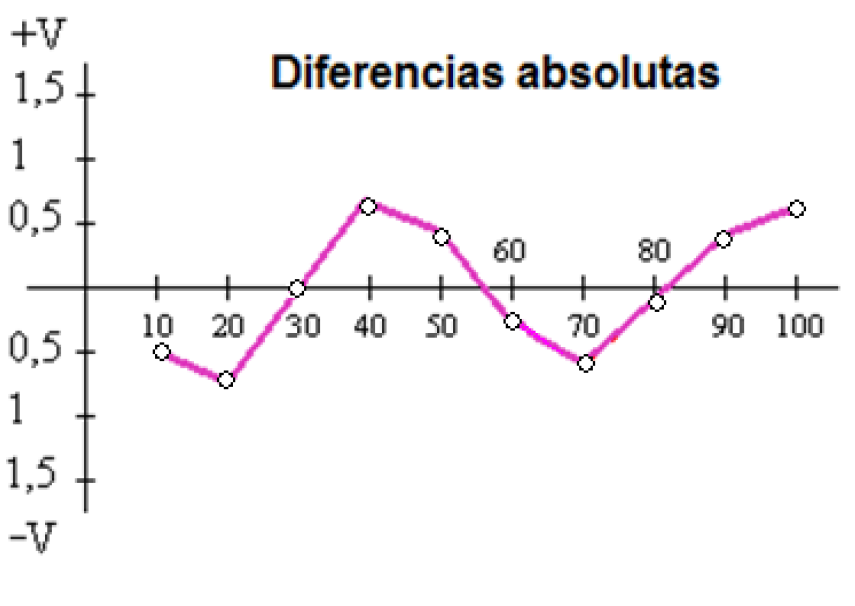
\includegraphics[width=0.6\linewidth]{imagenesTema2/absolut}
	\caption{Gráfica diferencias absolutas}
	\label{fig:absolut}
\end{figure}
	
	
	\item  \underline{\textbf{Curva de diferencias relativas}}: Permite valorar la importancia de cada error con respecto a la lectura. Los puntos se aproximan al eje conforme se avanza en el campo de medida.


\begin{figure}[H]
	\centering
	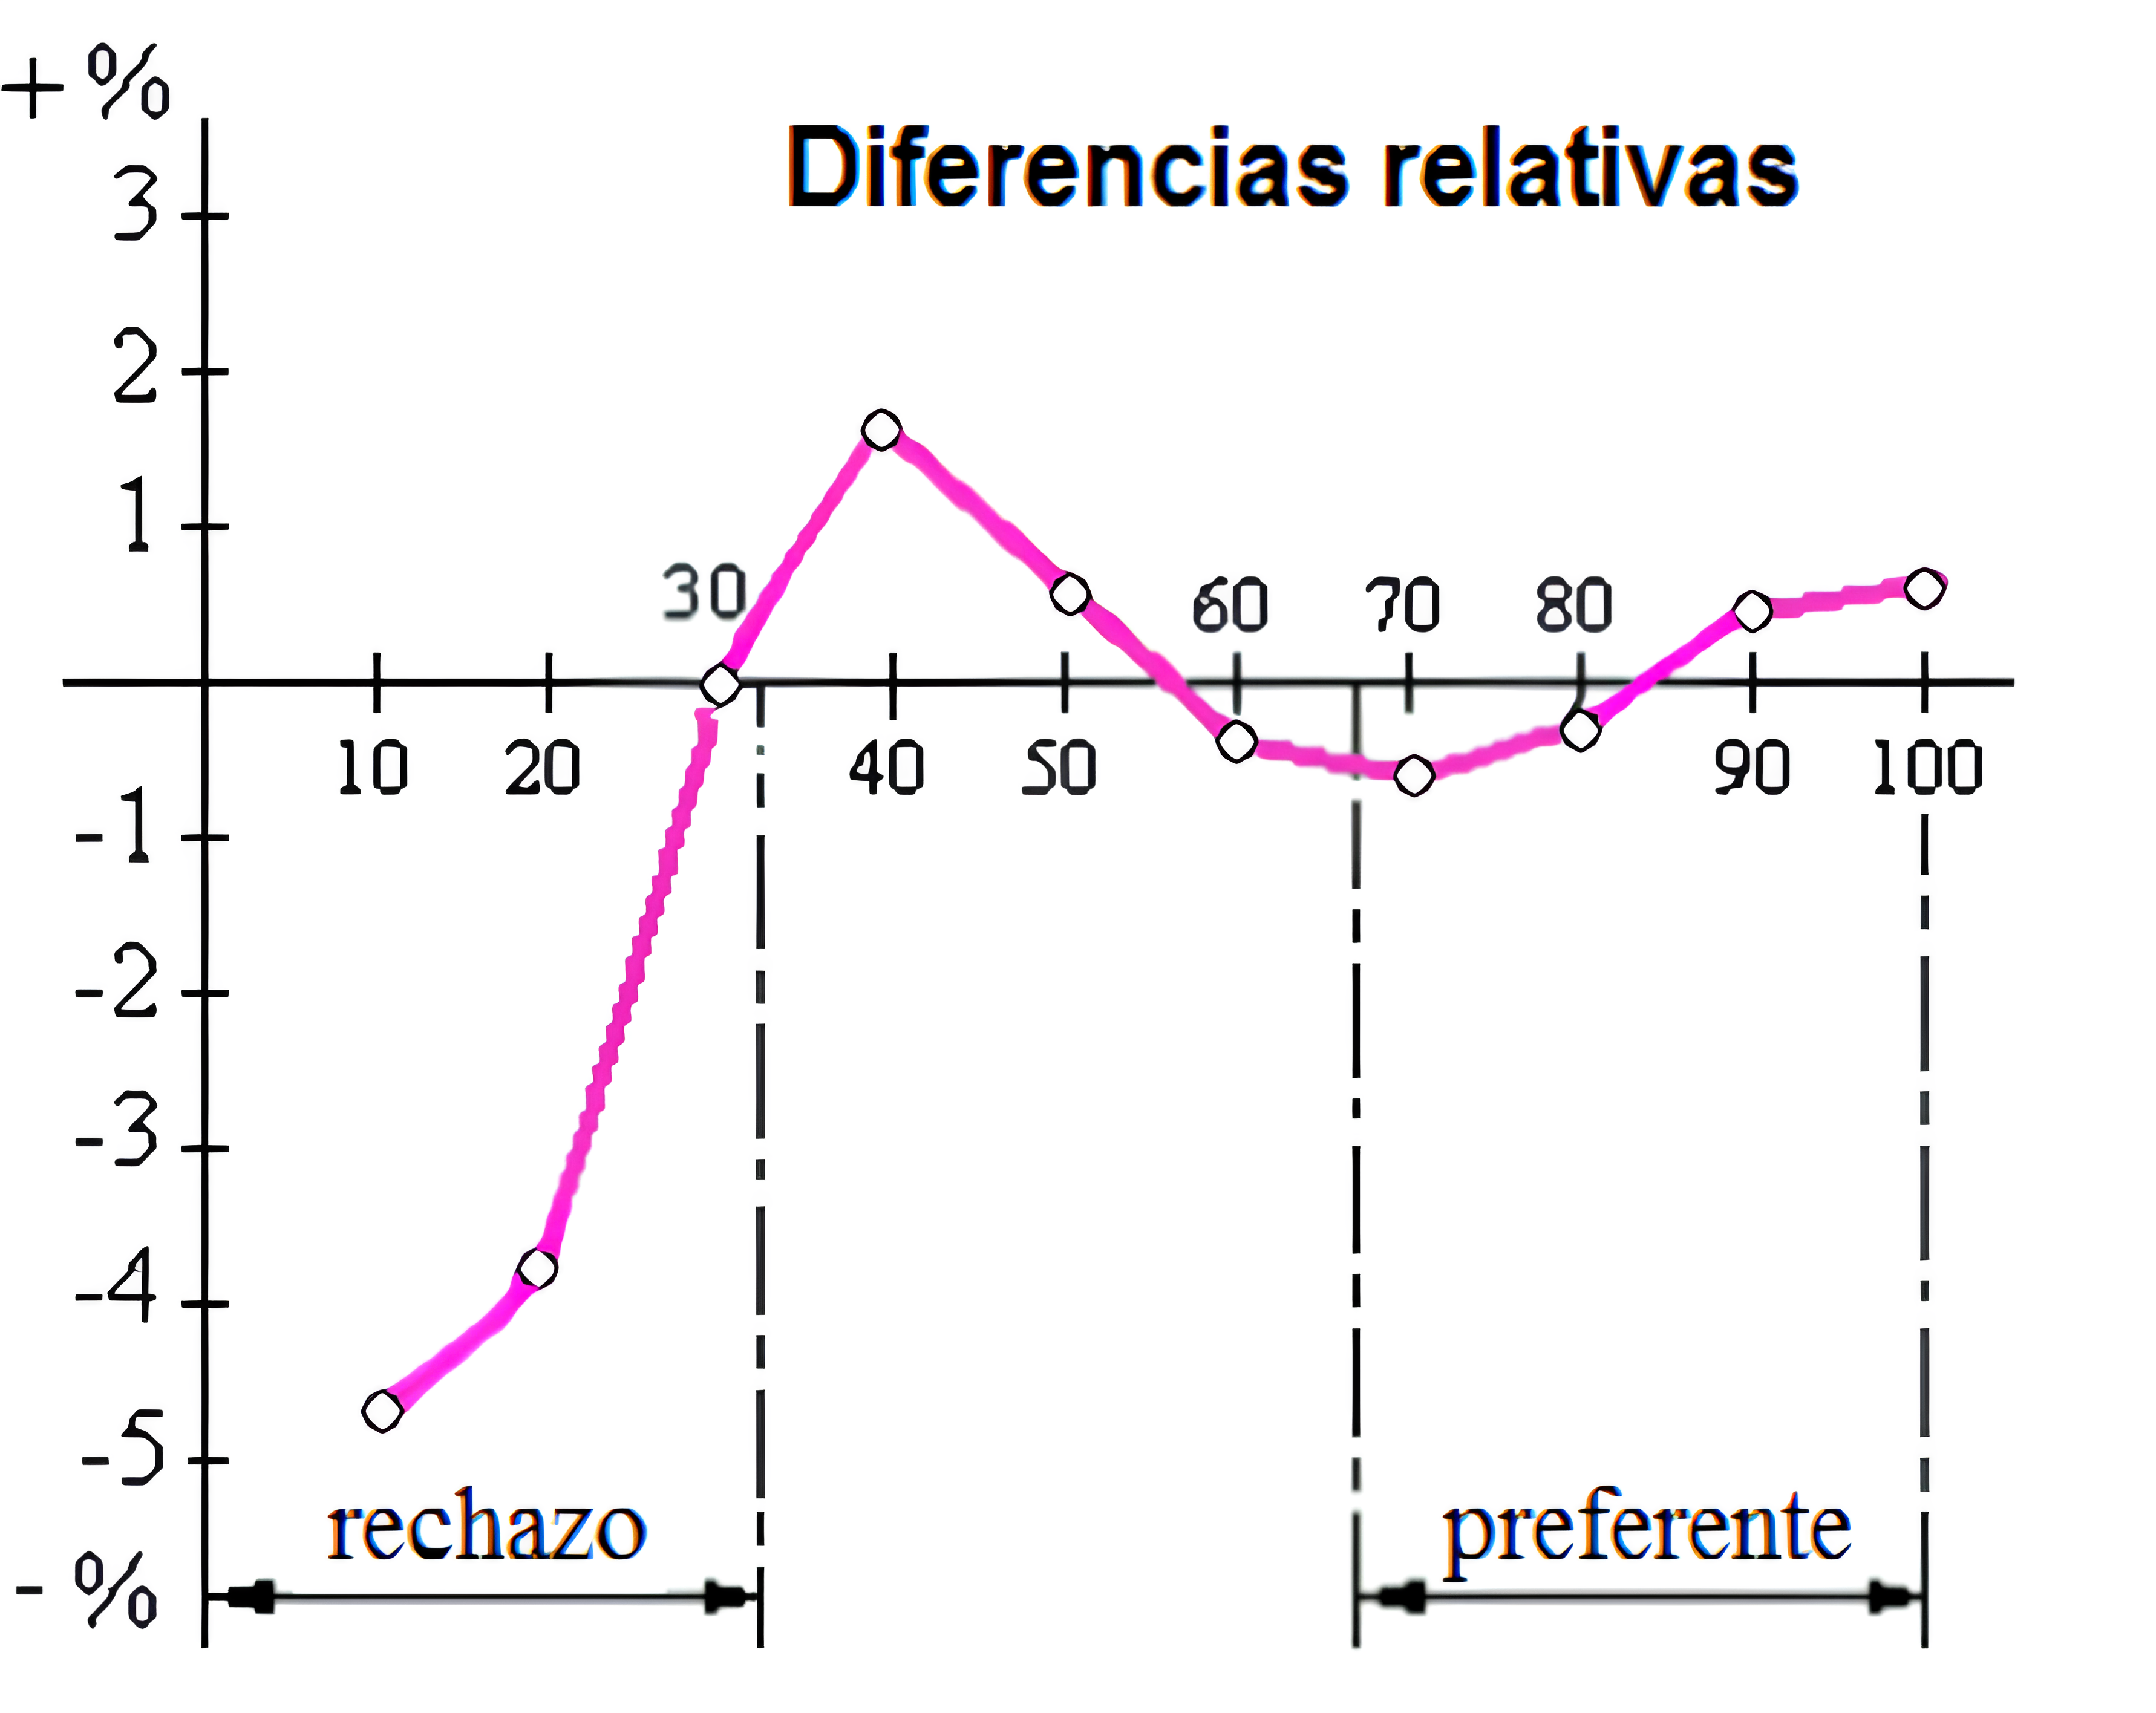
\includegraphics[width=0.6\linewidth]{imagenesTema2/relativo}
	\caption{Gráfica diferencias relativas}
	\label{fig:relativo}
\end{figure}





\end{enumerate}
\subsection{Incertidumbre de contraste}
\[U_c = \text{máx} \left[{k_c \ \sqrt[]{\frac{t^2 s_{ci}^2}{n_c}+\left({\frac{\bigtriangleup_i}{3}}\right)^2+u_p^2+u_{RC}^2+\text{Términos adicionales}}}\right]\]

\begin{itemize}
\item $k_c$ es el factor de cobertura.

	\item El factor t se obtiene de la tabla t student, si $n_c < 10$:
\renewcommand{\arraystretch}{1.1} %
\begin{table}[H]
	\centering
	\begin{tabular}{|c|c|c|c|c|c|c|c|c|c|}
		\hline
		\textbf{Número de medidas} & \textbf{2} & \textbf{3} & \textbf{4} & \textbf{5} & \textbf{6} & \textbf{7}
		& \textbf{8} & \textbf{9} & \textbf{10} \\
		\hline
		Factor t& 7.0 & 2.3 & 1.7 & 1.4 & 1.3 & 1.3 & 1.2
		& 1.2 & 1.1  \\
		\hline 
	\end{tabular}
	\caption{Tabla factor t student}
	\label{tab:example}
\end{table}

\item $s_{ci}$ es la desviación típica del punto de la escala $i$.
\item $\bigtriangleup_i$ es la diferencia respecto al patrón en el punto $i$.
\item $u_p$ incertidumbre sin expandir del aparato patrón:  $u_p=\frac{\alpha_p}{\sqrt{3}}$

\item $u_{RC}$ componente debida a la resolución del aparato contrastado.
\begin{itemize}
	\item Analógicos
	\[u_{RC}=\frac{E}{2\sqrt{3}} \ o \ u_{RC}=\frac{E}{4\sqrt{3}}\]
	
	\item Digitales
	\[u_{RC}=\frac{N dms}{2\sqrt{3}}\]
	
	\item $E$ es la división de una escala
	\item $N$ es un valor proporcionado por el fabricante. Normalmente $N = 1$
	\item $dms$ dígito menos significativo. 
\end{itemize}
\end{itemize}



\subsection{Clase de un aparato verificado}
El índice de clase facilita calcular incertidumbres. Permite fijar un límite de error máximo.

\[Clase=100 \frac{U_c (k=2)}{CM}\]

\subsection{Incertidumbre de la medida}
La incertidumbre al medir con el aparato calibrado será, donde el subíndice M denota de la muestra:

\[U_M=k_M \ \sqrt{u_c^2+t^2\frac{s_M^2}{n_m}+ \text{términos adicionales}}\]

No obstante, si se mide en condiciones similares a la de la calibración se habla de \textbf{capacidad óptima de medida (COM)} y se puede emplear la siguiente expresión:

\[U_M(COM)=k_M \ \sqrt{u_c^2+\frac{s_c^2}{n_m}+ \text{términos adicionales}}\]

Donde $s_c$ es la desviación típica de la contratación.


